\section{Repairs}

Most repairs follow one rule: an Earth value or a defect becomes a parameter whose default reproduces the
released code, so that the repair can be switched off and its effect compared with the original. Some
changes depart from the rule, and Table~\ref{tab:repairs} marks them. CM1's deeper soil and its zeroed trace
gases and ozone act in every patched build; its 400~ppm default for carbon dioxide replaces the calendar
formula, and the electrified build's gravity defaults to 9.81 where the released NSSL scheme has 9.8; the
beta plane's Coriolis force acts on departures from the base-state wind in beta-plane runs; the electrified
build caps the ice sizes its radiation reads; and SWAN's air density is compiled in. SWAN's wind-input patch
reproduces stock output only at standard gravity, 9.80665~m\,s$^{-2}$, set by input, and the guard added to
the water scaling is the identity only for spectra like the design case's. Each change is recorded as a patch
against a pinned upstream source, with its switch, its default and the checks made on it.

Three classes of repair differ in where their lunar values come from. A general repair corrects a unit,
applies a scaling law or a physical law, or removes a defect; its value follows from physics or from the
code's own intent, and another world takes it unchanged within the limits of Table~\ref{tab:reach}. A
general method with a per-world table computes a quantity of a world's own column, a path ratio or an energy
difference, and tabulates it, so the method serves another world once its table is computed there. A
calibration adjusts the free coefficients of an approximate scheme until its output matches the reference
model on chosen columns, and holds near the states it was fitted on. The line between the last two lies in
the tuning: the curved-air terms follow from the column's geometry and its computed radiation, while the
coefficients of the gas bands were fitted until PlaSim matched the line-by-line model's absorption. Beside
the three classes stand settings, which give the scenario's values; capabilities, which add a process or a
forcing the released codes lack; a bound, where the physics is unsettled; a mitigation; avoidances by
configuration; and a coupling method.

\textbf{Defects removed or avoided.} Patch 04 turns ExoPlaSim's Sun at the synodic rate continuously from the
first step, a mode that assumes a steady, non-synchronous rotation and counts the Sun's phase from step 0.
Patch 03 converts convective rain per 86,400~s. ExoPlaSim's own \code{fixedorbit} switch, whose documentation
describes only the freezing of Milankovitch variations, holds the configured orbit, and a year of 17,160
half-hour steps, twelve whole lunar model days, keeps output aligned with the Sun. SWAN's breaker parameter
is avoided by keeping depth-induced breaking on in every run, and SWAN's default initial state, whose 2~s
peak period has Earth's dimensions, by starting from rest or from hotstart files. The thread race and PlaSim's
cold lowest level stay open: CM1 runs that must repeat use one thread, and analyses of the lowest level
screen the cold windows.

\textbf{Constants to parameters.} The ExoPlaSim repairs are ten patches to PlaSim's radiation, cloud and Sun
code, each adding a namelist switch whose default is the released behaviour. In CM1, gravity and the air's
carbon dioxide and oxygen become preprocessor constants that default to 9.81~m\,s$^{-2}$, 400~ppm and
Earth's oxygen, and CM1's twenty spare namelist reals hold the lunar Sun, the forcing and the
electrification's settings. SWAN's wind-input knee moves with gravity and stays at 1~Hz under standard
gravity. The lunar runs were made with runners, the scripts that configure, compile and run each model, which
insert each change into the installed source at a marked anchor. The code repository holds the changes as
patch series against pinned upstream archives, and a script rebuilds from those archives, byte for byte,
the deployed ExoPlaSim installation and the Fortran of the eight lunar CM1 builds used for the results
reported here, while older CM1 builds, the Earth-gravity benchmark builds among them, were compiled from
earlier states of the series.\claim{R01}

\textbf{Scaling laws.} Where gravity enters a fitted law, a similarity argument gives the repair. A particle
falling in the regime $V = aD^b$ has a Reynolds number that grows as the Best number to the power
$(b+1)/3$ \autocite{mitchell1996use}, and the Best number of a particle of fixed size is proportional to
$g$, so $V \propto g^{(b+1)/3}$: at lunar gravity cloud droplets fall 6.04 times slower, raindrops 2.94 times
and graupel 2.27 times.\claim{R02} The scaling is exact for particles whose mass grows as $D^3$ and area as
$D^2$, as for drops, graupel and hail, within their fitted regimes; snow and ice crystals, whose mass and area
follow other powers, take a larger gravity exponent than the patch gives them. The Morrison and NSSL schemes
pass the scaled speeds through their fall-speed laws and caps into collection and ventilation, and in NSSL
the ventilation needed its own scaling at eleven sites.

The same argument sets other lengths and times. CM1's Rayleigh damping rate and its boundary-layer length
scale as $g$ and $1/g$, as the dynamics stretch, and WRF-ELEC's sub-step lengthens from 0.75 to 6.8~s, which
keeps graupel settling through about 1\% of a layer per sub-step in the 2~km layers of the lunar charging
zone, at 0.44 of Earth's fall speed; the boxes, rounding to whole sub-steps, run one 8~s sub-step per model
step.\claim{R03} The breakdown field already scales with the air's density, and lifting its
180~kV\,m$^{-1}$ cap lets that scaling act wherever lunar flashes start. SWAN's knee becomes a function of
$f\,g_\mathrm{E}/g$, which reproduces stock SWAN at standard gravity and restores the model's gravity
similarity.\claim{R04} The repairs of units and heights restore the quantity each formula was written for.
CCM3's cloud water counts heights and precipitable water at Earth's gravity and scales its mixing ratio by
$g/g_\mathrm{E}$, which gives each cloud the water path it would hold at the same pressures on Earth, and
CM1's five soil layers thicken to 5--80~cm, 1.55~m in all, deep enough for the thermal wave of any solar day
from a few Earth days to the Moon's.

\textbf{Geometry restored.} The curved geometry enters both models through an energy ledger of the design
column: the radiation of the same air traced once, offline, through spherical shells and through flat layers,
and the differences tabulated. For the ledger, sunlight from 360~nm to 5~\textmu m was traced through 100
spherical shells and through the same layers taken flat, at solar elevations from $-90$ to 90\textdegree, in
10,697 spectral channels. Each channel absorbs a direct beam within 1\% of its sunlight as its members do and,
beyond 1,250~nm, keeps the beam's loss above every layer; below 500~nm each band is one channel. The 282
channels below 1,250~nm thin enough to scatter take spherical successive orders of scattering from an in-house
sky solver, and the rest a direct beam through the shells with the diffuse light of a pseudo-spherical
two-stream, so their twilight lacks scattered light. The infrared escape is traced through the same shells by
impact parameter. The ledger's terms divide the curved geometry into the widening of the shells above each
square metre of ground, worth $-6.5$~W\,m$^{-2}$ net, and the curved light and escape, the twilight and the
low Sun's side light, worth $+0.7$~W\,m$^{-2}$.\claim{R05} Tabulated at 167 solar elevations from $-40$ to
90\textdegree, the terms add sunlight to each PlaSim layer or CM1 shell and the ground's share in the column's
clear share, below the horizon as well as above, and remove each layer's extra infrared escape, scaled with
temperature to the fourth power. PlaSim's slant factor becomes the Moon's, $(\mu+a)/(\mu^2+b\mu+c)$ fitted to
straight rays through the shells, within 0.30\% for water vapour and 0.08\% for well-mixed air
(Figure~\ref{fig:slant}).\claim{R06} Part of the daylight term is a difference of solvers: with the Sun
overhead, where the geometry is flat, the spherical solver's ground still takes 1.3\% less than the
two-stream's, so the daytime term also corrects the reference column PlaSim was calibrated against.\claim{R07}

\begin{figure}[tbp]
\centering
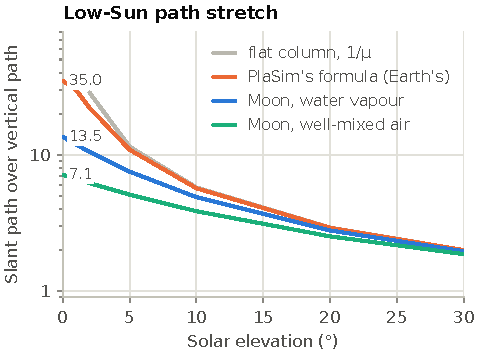
\includegraphics[width=0.6\textwidth]{figures/fig_slant.pdf}
\caption{The slant path over the vertical path as the Sun nears the horizon. PlaSim's formula,
$35/\sqrt{1+1224\mu^2}$, has Earth's horizon value; the Moon's factors for water vapour and for well-mixed
air come from straight rays through the design column's shells. The flat column's $1/\mu$ diverges at the
horizon.}
\label{fig:slant}
\end{figure}

\textbf{Calibration by height.} PlaSim was calibrated against the in-house radiative--convective model and
its correlated-$k$ emulation. The model is clear-sky and line-by-line, built on HITRAN lines of water, carbon
dioxide and oxygen as served in September 2026 (HITRAN2020 or a later edition), a re-implementation of
MT\_CKD~4.3, collision-induced absorption and Rayleigh scattering, with gravity falling as $GM/r^2$ and a
pseudo-spherical direct beam; its emulation reproduces the outgoing longwave within 0.4~W\,m$^{-2}$ at
288--290~K and within 1.4~W\,m$^{-2}$ for a saturated 330~K lunar column.\claim{R08} Each calibration was made
to remove the residual of the one before. The first fitted two totals, a Rayleigh multiplier and a weaker
water continuum on global-mean columns, which brought the clear-sky albedo within 0.007 and the outgoing
longwave within about 2~W\,m$^{-2}$. Once the Sun-clock and orbit defects were found, a check of how each
column split its own arriving sunlight showed the air 7.7--8.2 points short, and a multiplier on the
near-infrared water absorptivity, refitted with the Rayleigh multiplier on eleven columns, brought the split
within 0.3 points rms.\claim{R09} By layer the fit still placed sunlight low: PlaSim put almost nothing above
85~km, where the line-by-line column absorbs 4.2~W\,m$^{-2}$. Three carbon dioxide and oxygen bands, each
fitted to the line-by-line beam's loss above every level within 0.13\% of its energy, and a refit of both
multipliers brought the layers within 0.97~W\,m$^{-2}$ rms of the reference, from 1.71
(Figure~\ref{fig:layers}).\claim{R10} In the longwave, a fit to totals proved insufficient: PlaSim's water
continuum had been fitted to the outgoing flux, which a scheme can match while misplacing its cooling by
10~W\,m$^{-2}$ in a layer. An extra escape to space for each layer and for the ground, fitted over land and
over sea on about 2,100 cloud-free three-day means and scaled with temperature to the fourth power, removes
each layer's mean error and leaves 1--5~W\,m$^{-2}$ from column to column.\claim{R11}

\begin{figure}[tbp]
\centering
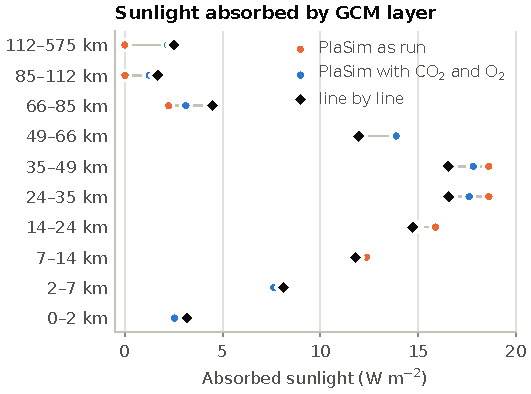
\includegraphics[width=0.62\textwidth]{figures/fig_layers.pdf}
\caption{Sunlight absorbed in each GCM layer of the design column, global means: the line-by-line
pseudo-spherical model against PlaSim's arithmetic on the same column as run, and with the carbon dioxide
and oxygen bands and the refitted multipliers. With the bands the layers come within 0.97~W\,m$^{-2}$ rms of
the reference, against 1.71 as run; about 2~W\,m$^{-2}$ of water's sunlight still lands at 35--66~km in
place of 66--85~km and the lowest 7~km.}
\label{fig:layers}
\end{figure}

\textbf{Processes and capabilities added.} Cloud colder than $-38$\,\textdegree C takes Ebert and Curry's ice
optics \autocite{ebert1992parameterization} through a delta-scaled two-stream, with an effective radius from
Kristjánsson and Mitchell's table \autocite{kristjansson2000impact}, in place of liquid water's, a physical
law in place of a simplification. WRF-ELEC's charge separation, discharge and screening, which CM1 lacks,
were grafted into it: the NSSL scheme with charge on every hydrometeor; a Poisson solver by Fourier transform
across the periodic domain and a tridiagonal solve on CM1's stretched levels; WRF-ELEC's cylindrical
discharge \autocite{ziegler1994observed} and its three-dimensional discharge adapted from
\textcite{macgorman2001lightning}, on a domain that wraps round; and its screening layers, available and off
in the lunar runs.\claim{R12} The lunar runs add leakage of charge through a computed lunar conductivity
column, and a leader's crossing to the ground at an internal field of 1~kV\,m$^{-1}$ at sea-level density,
scaled with the air's density, which places the ground strikes between the bounds set by WRF-ELEC's stopping
field and its $-7$\,\textdegree C rule; point discharge from the ground, added as an option, ran in one test
window and stays off.\claim{R13} PlaSim gains a downward infrared flux at the model top, by day and by night,
for any source above the air, a host planet's glow for a moon among them, and CM1's radiation reads ice sizes
capped at RRTMG's 140~\textmu m, with the excess logged.

\textbf{Forcing a slice of the GCM.} Running CM1 inside the GCM's climate adds a structural limit to the
inherited ones: a ring of columns along a latitude circle lacks the transport across the circle, a box lacks
any day--night circulation larger than itself, and stock CM1 has no lunar Sun, no forcing above its
boundary layer and no nudging that follows terrain. Two of these absences showed in the runs. The first box,
forced with the advection along the rings alone, rained in the mornings and stayed clear and hot in the
afternoons until it was stopped at day 47, and at 45\textdegree\,N the missing transport across the circle
accounts for about a third of CM1's warm offset from the GCM.\claim{H32} The forcing methods supply what the
slice lacks from the GCM's fields, and with them the GCM's remaining Earth values. Each ring column has its own
Sun (a box takes one) and, on tilted rings, its own Coriolis parameter; CM1 is nudged toward the GCM only above
8--16~km, so its boundary layer and convection develop freely, and the GCM's mean vertical wind enters CM1's
own large-scale advection.\claim{R14} A heating and moistening by local time and height supplies the
day--night circulation a box lacks and, as a single local-time bin, the transport across the circle a ring
lacks; over terrain each column is nudged and forced at its own height above sea level. SWAN takes the GCM's
surface stress through Wu's drag law inverted to an equivalent wind, so its friction velocity matches the
GCM's to within a few per cent, on spherical coordinates at the lunar radius and with its frequency band
scaled by $g/g_\mathrm{E}$; SWASH, unmodified, takes lunar gravity as an input and SWAN's spectra at its
boundary.\claim{R15}
